\documentclass[a4paper]{scrartcl}

\usepackage[ngerman]{babel}
\usepackage[utf8]{inputenc} 
\usepackage{amsmath}
\usepackage{amssymb}
\usepackage{enumerate}

\selectlanguage{ngerman}

\usepackage[pdftex]{graphicx}

\usepackage{empheq}

\usepackage{todonotes}

\usepackage[a4paper,left=2.5cm,right=2.5cm,top=2.5cm,bottom=2.5cm]{geometry} 

\usepackage{color}

\definecolor{rot}{cmyk}{.4,1,1,0}   % hellroter Text

%befehl damit tag in align umgebung mit klammer über zwei zeilen möglich ist
\newcommand{\smarttag}[1]
{
 \tag*{\makebox(80,0){\rule[4ex]{0pt}{1ex}$\bigg.\bigg\}${#1}}}
}
\newcommand{\Smarttag}[1]
{
 \tag*{\makebox(80,0){\rule[10ex]{0pt}{1ex}$\Bigg.\Bigg\}${#1}}}
}

%werden wir sicher öfter brauchen
\newcommand{\Fhat}{
\hat{\mathbb{F}}
}
\newcommand{\F}{
\mathbb{F}
}
\newcommand{\Fhatfunc}[1]{$\Fhat$\,(#1) }
\newcommand{\LandauO}{\mathcal{O}}
\newcommand{\Landauo}{\scriptstyle \mathcal{o}}

% workaround damit zeilenumbruch nach paragraph erfolgt
\newcommand{\example}[1]{\subparagraph{#1}$\;$ \\ }
\newcommand{\para}[1]{\paragraph{#1}$\;$ \\ }


\begin{document}
\title{Technische Numerik \\ Mitschrift}
\author{A. Schwarzl, C. Sirk}
\maketitle

\tableofcontents

\section{Einführung - 3.10.2012}

Numerische Mathematik befasst sich mit der näherungsweisen Lösung von Problemstellungen (mit dem Computer).
%\begin{itemize}
  %\item Formulierung
  %\item Entwicklung
  %\item Untersuchung
  %\item Implementierung
    %von Verfahren und Algorithmen
%\end{itemize}
\begin{equation*} 
  \left.
  \begin{aligned} 
   & \text{Formulierung} \\ 
   & \text{Entwicklung} \\ 
	 & \text{Untersuchung} \\
 	 & \text{Implementierung} \\
  \end{aligned} 
  \right\} 
  \text{von Verfahren und Algorithmen} 
\end{equation*} 
Von der Problemstellung zur Näherungslösung:

  \begin{empheq}{alignat*=3} 
   & \text{physikalisches, chemisches, ... Problem bzw. Modell} & \smarttag{Modellfehler} \\ 
   & \text{mathematisches Modell (z.B. DGL)} & \smarttag{Diskretisierungsfehler} \\ 
	 & \text{numerisches Näherungsverfahren (endlich} & \Smarttag{Verfahrensfehler}\\
	 & \text{ dim. Ersatzproblem)} \\
 	 & \text{Algorithmen für Ersatzprobleme} & \smarttag{Impl.-fehler z.B. Rundungsfehler}\\
	 & \text{Implementierung} & \\
  \end{empheq}
Die letzten drei Punkte werden von der Numerik abgedeckt.\\
\textbf{ZIEL}: (möglichst) genau, möglichst schnell, mit möglichst geringem Aufwand (z.B. Speicher)

\subsection{Gleitpunktzahlen $\Fhat$}
\begin{align*}
		\Fhat = \F \cup \F_d \hspace{0.5cm} \text{mit} \hspace{0.5cm} & \F && \text{normalisierte Gleitpunktzahlen}\\
		 &\F_d && \text{denormalisierte Gleitpunktzahlen} 
\end{align*}
\para{Normalisierte GPZ}

\begin{align*}
x = \sigma\,\cdot\,M\,\cdot\,\,b^e \hspace{0.5cm} \text{mit} \hspace{0.5cm} & \sigma && \text{Vorzeichen}\\
& M && \text{Mantisse} \\
& b && \text{Basis} \\
& e && \text{Exponent}
\end{align*}

\begin{align*}
M = \sum^t_{k=1} d_k b^{-k} \hspace{0.5cm} \text{mit} \hspace{0.5cm} & d_1,\ldots,d_t\, \in\,\{0,1,\ldots,b-1\} && \text{Ziffern der Mantisse}\\
& t && \text{Mantissenlänge} \\
& d_1 \neq 0 && \text{(Normalisierung)} \\
& e_{min} \leq e \leq e_{max} && \text{Exponentenbereich}
\end{align*}

Schreibweise:
\begin{equation*}
x = \sigma\,(0.d_1d_2d_3\,\ldots\,d_t)b^e
\end{equation*}

\para{Denormalisierte GPZen}
\begin{figure}[htbp]
  \centering
  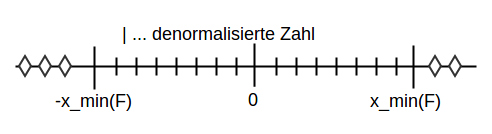
\includegraphics[width=0.7\textwidth]{figures/denormalisiertezahlen.png}
  \caption{Zahlenstrahl mit denormalisierten und normalisierten Zahlen}
  \label{fig:denormalisiert}
\end{figure}

\begin{align*}
x_d = \sigma\,M\,b^{e_{min}} &\\
M = \sum^t_{k=2} d_k b^{-k} \hspace{0.5cm} \text{mit} \hspace{0.5cm} & d_2,\ldots,d_t\, \in\,\{0,1,\ldots,b-1\} \\
& \text{keine Normierung} 
\end{align*}

\para{Gleitpunktzahlsystem}
\Fhatfunc{b,t,$e_{min}$,$e_{max}$}

\example{Beispiel: "`Doppeltes Grundformat"' ("`double"' in C, Java, MATLAB)}

\Fhatfunc{2,\,53,\,-1021,\,1024} Im PC als 64bit $\rightarrow$ 52 + 1 da erstes bit ungleich 0 sein muss, 11 Stellen für Exponenten / Umschaltung zu denorm. GPZ. Symbolische Ausdrücke ("`Inf"',"'NaN"',...) 
kleinste/größte pos Zahl:
\begin{align*}
	& x_{min}(\F) =  2^{-1022}\,\approx\, 2,23\cdot\,10^{-308} \\
	& x_{max}(\F) \approx 1,8\,\cdot\,10^{308} \\
  & x_{min}(\Fhat) \approx 5\cdot\,10^{-324} & \text{nicht in diesen Bereich gehen!}
\end{align*}

\subsubsection{Rundung}
Die Abbildung $rd: \mathbb{R} \rightarrow \Fhat, x\,\mapsto\,rd(x)$ heißt Rundung, wenn $|rd(x)-x|=min|y-x|, y\in\,\F$. 
\todo{realtiver Fehler unterbringen}
\begin{empheq}[innerbox=\fbox,right=\Leftarrow{\text{gilt nur für normalisierte Zahlen}}]{align*}
\text{Für} \hspace{1cm} x_{min}(\F)&\leq\,|x|\,\leq\,x_{max}\,(\F) \hspace{1cm}\text{gilt:}\\
\frac{|rd(x)-x|}{x}&\leq \frac{1}{2}\,b^{-t+1} \eqqcolon eps \leftarrow \text{Maschinengenauigkeit}
\end{empheq}

Es sei $\frac{rd(x)-x}{x}=\sigma\,\Rightarrow\,rd(x)=x(1+\delta)$
es gilt:
\begin{empheq}[innerbox=\fbox]{align*}
rd(x)=x(1+\delta) & \hspace{1cm} |\delta|\leq\,eps
\end{empheq}

\example{Maschinengenauigkeit für "`double"'}
\Fhatfunc{2,\,53,\,-1021,\,1024}
\begin{equation*}
eps = \frac{1}{2}\,2^{-53+1}\approx\,1,1\cdot\,10^{-16}
\end{equation*}
Maschinenepsilon 
\begin{equation*}
\epsilon_M=2 eps = b^{-t+1}
\end{equation*}

$\epsilon_M$ ist der Abstand zwischen 1 und der nächstgrößeren GPZ.

\subsubsection{Gleitpunktarithmetik}
Schon elementare Operationen von GPZen führen zu Resultaten, die nicht im $\Fhat$
liegen, zB $\frac{1}{3} \not \in \Fhat$. \\
Maschinenoperationen: $\oplus$, $\ominus$, $\odot$, $\oslash$ \\
Genaue Operation: $\Box$ \\
Standard für die Genauigkeit von Maschinenoperationen (IEEE 754): \\

\begin{empheq}[innerbox=\fbox]{align*}
 x \circ y &= rd(x \Box y)   \\ 
\text{für} \hspace{0.5cm} x, y \in \Fhat, x_{min}(\F) &\leq | x \circ y | \leq x_{max}(\F)\\
  & \Updownarrow \\
 x \circ y & = (x \Box y)(1 + \delta) \hspace{0.5cm} \text{mit} \hspace{0.5cm} |\delta | \leq eps
\end{empheq}

\subsubsection{Fehlerverstärkung bei elementaren Rechenoperationen}
Fragestellung: Wie wirken sich fehlerbehaftete Eingangsdaten bei elementaren
Rechenoperation aus? Kann es zu einer wesentlichen Fehlerverstärkung kommen?
Ja, es kommt aber darauf an.
\example{Bsp:}
$ f(x)=\frac{1 - \cos(x)}{x^2} $ für $x=1.2 \cdot 10^{-5} $
Angenommen wir runden $\cos(x)$ auf 10 Stellen genau \\
\begin{align*}
 \cos(x) &\approx 0.999 999 999 9 =: c \\
 \frac{1 - c}{x^2} &= \frac{10^{-10}}{1.44 \cdot 10^{-10}} = 0.6944\dots 
\end{align*}
Mit Hilfe der Taylorreihe lässt sich zeigen, dass $ f(x) \in [0, \frac{1}{2}) $. \\
relativer Fehler $ \geq \frac{0.69 - 0.5}{0.5} = 38\% $ \\

\para{Fehlerverstärkung bei Addition (Subtraktion)}
Seien $ a, b \in \mathbb{R} $ gegeben und
$ \tilde{a} = rd(a) = a (1 + \delta_{a}) $ mit $ | \delta_{a} | \leq eps $ sowie
$ \tilde{b} = rd(b) = b (1 + \delta_{b}) $ mit $ | \delta_{b} | \leq eps $ \\
Relative Fehler\\
\begin{equation*}
\left| \frac{\tilde{a} + \tilde{b} - (a + b)}{a + b} \right| =
\left| \frac{a\delta_{a} + b\delta_{b}}{a + b} \right| \leq eps \frac{|a| + |b|}{|a + b|} 
\end{equation*}
Ist $ |a + b| \ll |a| + |b| $ dann kann der relative Fehler groß werden.
D.h. bei der Subtraktion zweier annähernd gleich großer Zahlen, können
sich Eingangsfehler erheblich verstärken. $\Rightarrow$ \large{\textcolor{rot}{\textbf{AUSLÖSCHUNG
signifikanter Stellen}}}

\para{Fehlerverstärkung bei Multiplikation}
Seien $ a, b \in \mathbb{R}\setminus\{0\} $ gegeben und
$ \tilde{a} = rd(a) = \frac{a}{1 + \delta_{a}} $ mit $ | \delta_{a} | \leq eps $ sowie
$ \tilde{b} = rd(b) = \frac{b}{1 + \delta_{b}} $ mit $ | \delta_{b} | \leq eps $ \\
Relative Fehler
\begin{gather*}
\left| \frac{\tilde{a}\tilde{b} - a b}{a b} \right| =
\left| \frac{\frac{ab}{(1 + \delta_{a})(1 + \delta_{b})} - ab}{ab}\right| = \\
\left| \frac{ab - ab(1 + \delta_{a})(1 + \delta_{b})}{ab(1 + \delta_{a})(1 + \delta_{b})} \right| =
\left| \frac{ab(\delta_{a} + \delta_{b} + \delta_{a}\delta_{b})}{ab(1 + \delta_{a})(1 + \delta_{b})} \right| \leq
\frac{3eps}{1 - 3eps} \leq 4eps 
\end{gather*}
$\Rightarrow$ Multiplikation führt nicht zu einer wesentlichen Fehlerverstärkung.
Dasselbe lässt sich auch für die Division zeigen.

\subsection{Landau-Symbole (``$\LandauO$-Notation'')}
Verwendung zur:
\begin{itemize}
  \item Beschreibung des asymptotischen Verhaltens von Funktionen
  \item Effizienzverhalten von Algorithmen
\end{itemize}
Definition: Seien $f,g: \mathbb{R} \to \mathbb{R}$
\begin{enumerate}[(a)]
  \item $f(x) = \LandauO(g(x))$ für $x \to a :\Leftrightarrow$
    Es gilt $c > 0$ und $\delta > 0$, so dass für alle $x \in \{|y - a| < \delta\}: |f(x)| \leq c|g(x)| \Leftrightarrow$ in etwa ähnliches Verhalten
  \item $f(x) = \LandauO(g(x))$ für $x \to \infty :\Leftrightarrow$
    Es gilt $c > 0$ und ein $x_0 > 0$, so dass für alle $x > x_0:\,|f(x)| \leq c|g(x)| \Leftrightarrow$ $f(x)$ wächst nicht schneller als $g(x)$
  \item $f(x) = o(g(x))$ für $x \to \Box \in \mathbb{R} \cup \{\pm \infty\} :\Leftrightarrow
    \underset{x \to \Box}{\lim}|\frac{f(x)}{g(x)}| = 0$
\end{enumerate}

\example{Beispiel:}
\begin{align*}
  \frac{x + 1}{x^2} &= \LandauO(\frac{1}{x}) \text{ für } x \to \infty \text{ , denn } \\
  \frac{1}{x} + \frac{1}{x^2} &\leq \frac{1}{x} + \frac{1}{x} = \underbrace{2}_c \frac{1}{x} \text{ für } x \geq \underbrace{1}_{x_0}
\end{align*}
\begin{align*}
  x^{\alpha} = o(x^{\alpha + 1}) \text{ für } x \to \infty \text{ , denn }
  \frac{x^{\alpha}}{x^{\alpha + 1}} = \frac{1}{x} \xrightarrow[x\to\,\infty]{}0
\end{align*}
\textcolor{rot}{VORSICHT}: Das Gleichheitszeichen ist bei Verwendung der Landau-Symbole rein symbolisch
zu verstehen: Symmetrie $[a = b \Leftrightarrow b = a]$ und Transitivität 
$[a = b \wedge b = c \Rightarrow a = c]$ gelten i.A. nicht. \\
z.B.: $x = \LandauO(x^2)$ für $x \to \infty$ aber $x^2 \neq \LandauO(x)$ für $x \to \infty$

\subsection{Fehleranalyse}
Bei der Analyse der Fehlerfortpflanzung bei der Lösung von mathematischen Problemen
unterscheidet man:
\begin{itemize}
  \item Kondition des Problems
  \item Stabilität des Algorithmus (zur Lösung des Problems)
\end{itemize}
\para{Kondition eines Problems}
Mathemathisches Problem sei durch eine Funktion beschrieben: $H:X \to Y$ \\ 
$\underbrace{x}_{\textrm{Input}} \mapsto \underbrace{H(x)}_{\textrm{Resultat}}$\\
Fehlberbehafteter Input $x + \Delta x$ mit $\Delta x$ als Fehler
\begin{align*}
  \frac{|| H(x + \Delta x) - H(x)||}{|| H(x) ||} = ?
\end{align*}
\para{Satz von Taylor (Taylorreihenentwicklung):}
\begin{enumerate}[(a)]
  \item Sei $f: I \in \mathbb{R} \to \mathbb{R}\,$ (n + 1)-mal stetig differenzierbar, dann gilt für
    $x, \Delta x \in I$: \\
    $f(x + \Delta x) = f(x) + \Delta x f^{\prime}(x) + 
    \frac{(\Delta x)^2}{2!}f^{\prime\prime}(x) + \ldots + 
    \frac{(\Delta x)^n}{n!}f^n(x)+
    \frac{(\Delta x)^{n + 1}}{(n + 1)!}f^{n + 1}(\zeta(x)) $ \\
    wobei $x \leq \zeta(x)\leq x + \Delta x$
  \item Sei $f: \mathbb{R}^n \to \mathbb{R}^m\,$ 2 mal stetig differenzierbar \\
    $f(x + \Delta x) = f(x) + \Delta x f^{\prime} + R(x, \Delta x) $ \\
    wobei $||R(x, \Delta x)|| = \LandauO(||\Delta x||^2)$ für $||\Delta\,x|| \to 0$
\end{enumerate}

\para{Absoluter Fehler:}
$\Delta H(x) := H(x + \Delta x) - H(x)$ wenn $||\Delta x|| \ll 1$ ist, dann \\
$\Delta H(x) \cong H^{\prime} \Delta x$

\para{Relative Fehler (1D Fall):}
\begin{align*}
  \delta H(x) := \frac{\Delta H(x)}{H(x)} \mathrel{\widetilde{=}} 
  \frac{H^{\prime} \Delta x}{H(x)} =
  \frac{x H^{\prime}(x)}{H(x)} \cdot \frac{\Delta x}{x}
\end{align*}
Verstärkerfunktion $=: \kappa(H, x) = | \frac{x H^{\prime}(x)}{H(x)} |$ \\
relative Eingangsfehler $:= \delta x = \frac{\Delta x}{x}$
\begin{empheq}[innerbox=\fbox]{align*}
  |\delta H(x)|  \cong \kappa(H, x) |\delta x|
\end{empheq}
$\kappa(H, x)$ wird (relative) Kondition(szahl) des Problems $H$ für den Input $x$
genannt. (Mehrdimensionaler Fall: Analoge Definition; verwende Normen statt Beträge) \\
Ein Problem heißt \underline{gut konditioniert}, falss die Konditionszahl klein (nahe bei 1) ist
(für die infragekommenden Inputs).

\example{Beispiel:}
Die Nullstellen der quadratischen Gleichung $\lambda^2 - 2x\lambda + 1 = 0$ sind für $x > 1$ gegeben durch 
$\lambda_1 = x +\sqrt{x^2 - 1} \;\;\; \lambda_2 = x - \sqrt{x^2 - 1}$ \\
Konditionszahl für $\lambda_2 = H(x)$
\begin{align*}
  \kappa(H, x) = \left|\frac{x H^{\prime}(x)}{H(x)}\right| = 
  \left|\frac{x[1 - \frac{1}{2}(x^2 - 1)^{-\frac{1}{2}} 2x]}{x - \sqrt{x^2 - 1}} \right| =
  \left|\frac{\frac{x(\sqrt{x^2 - 1} - x)}{\sqrt{x^2 - 1}}}{x - \sqrt{x^2 - 1}}\right| =
  \left|- \frac{x}{\sqrt{x^2 - 1}}\right|
\end{align*}
Fallunterscheidung:
\begin{enumerate}[(i)]
  \item $x \gg 1:\ \kappa(H, x) \approx 1 \Rightarrow$ gut konditioniert
  \item $x \approx 1:\ \kappa(H, x)$ groß $\Rightarrow$ schlecht konditioniert
\end{enumerate}
Berechnung der Lösung für i)
\begin{enumerate}[(a)]
  \item $H(x) = x - \sqrt{x^2 - 1}$ numerisch instabil (Auslöschung)
  \item $H(x) = \frac{(x - \sqrt{x^2 - 1})(x + \sqrt{x^2 - 1})}{x + \sqrt{x^2 - 1}} = $
    $\frac{1}{x + \sqrt{x^2 - 1}}$ numerisch stabil
\end{enumerate}

\para{Stabilität eines Algorithmus}
Dafür gibt es verschiedene uneinheitliche Konzepte und Definitionen. \\
\underline{Komperative Erklärung}: \\
Algorithmus I zur Lösung eines Problemes ist stabiler als Algorithmus II,
wenn der Gesamteinfluss der Rundungsfehler bei Algorithmus I kleiner als
bei Algorithmus II ist.


%\section{Approximation von Funktionen}
% hat er es nur umbenannt?, ja glaub schon
\section{Interpolation}
Aufgabenstellung: Aus einer festgelegten Menge von Funktionen $M_n$ 
bestimme man eine Funktion, die durch die gegebenen Punkte
$(x_0, f_0), (x_1, f_1), \cdots, (x_n, f_n) \in \mathbb{R}^2$ verläuft.

\missingfigure{Funktion mit Stützstellen}
Die Wahl von $M_n$ ist abhängig von der Problemstellung:
\begin{itemize}
  \item $\Pi_n$: Menge der Polynome mit Grad $\leq$ n
  \item stückweise polynomiale Funktion
  \item trigonometrische Funktion
	\item $\cdots$
\end{itemize}
Warum und weshalb:
\begin{itemize}
  \item Berechnung von Zwischenwerten einer Funktion, die nur an wenigen 
    Stellen bekannt ist
  \item Vereinfachung der Komplexität einer Funktion. (Beschreibung
    einer Funktion durch eine kleine Anzahl von Funktionen) $\Rightarrow$
    einfacheres Rechnen
  \item wichtige theoretische Grundlage für verschiedene andere numerische
    Aufgaben (Integration, Differenzialgleichungen)
\end{itemize}

\subsection{Polynominterpolation}
\underline{Gegeben}: Paarweise verschiedene Stützstellen $x_0, x_1, \cdots x_n$ und
Werte $f_0, f_1, \cdots f_n$.\\
\underline{Gesucht}:
\begin{equation*}
  \tag{2.1} p_n \in  \Pi_n \text{, so dass } p_n(x_i) = 
  f_i \text{ für } i = 0, 1, \cdots ,n
\end{equation*}
Grundlegende Fakten zu Polynomen:
\begin{enumerate}[(i)]
  \item $\Pi_n$ die Menge der Polynome mit Grad $\leq$ n ist ein Vektorraum
  \item Die Monome $1, x, x^2, \cdots, x^n$ bilden eine Basis von $\Pi_n$
  \item Polynom von Grad n $\geq$ 1 mit komplexen Koeffzienten besitzt genau n-Nullstellen
    in $\mathbb{C}$, wobei die Anzahl der Nullstellen entsprechend der Vielfachheit
    gezählt wird.
\end{enumerate}
\paragraph{Satz:} Die Polynominterpolationsaufgabe (2.1) ist eindeutig lösbar\\
Beweis:
\begin{enumerate}[(a)]
  \item Eindeutigkeit: Angenommen $p_n, q_n \in \Pi_n$ erfüllen (2.1), d.h. $p_n(x_i)=q_n(x_i)=f_i $für i=0,1,...n\\
    $r := p_n - q_n \in \Pi_n$ \\
    $r(x_i) = 0$ für $i = 0, \cdots, n \Rightarrow r$ hat $n + 1$ Nullstellen
    $\Rightarrow r \equiv 0 \Rightarrow p_n \equiv q_n$
  \item Existenz: Konstruiere Polynome $L_0(x), L_1(x), \cdots, L_n(x) \in \Pi_n$ mit\\
    $L_i(x_k)=\begin{cases} 1 & \mbox{für } \mbox{ $i = k$} \\ 
      0 & \mbox{sonst} \end{cases}$ \\
    $\Rightarrow L_i$ hat n Nullstellen: $x_0, x_1, \cdots, x_{i-1}, x_{i+1}, \cdots, x_n$
		\begin{align*}    
		L_i \in \Pi_n \Rightarrow L_i(x) = a(x-x_0)(x-x_1)\cdots(x-x_{i-1})(x-x_{i+1})\cdots(x-x_n)\\
    L_i(x_i) \overset{!}{=} 1 \Rightarrow
      a = \frac{1}{(x_i-x_0)(x_i-x_1)\cdots(x_i-x_{i-1})(x_i-x_{i+1})\cdots(x_i-x_n)}\\
    \end{align*}
		\begin{empheq}[innerbox=\fbox,right=\Leftarrow{\text{LAGRANGE-POLYNOME}}]{align*}
		\Rightarrow L_i(x) = \frac{(x - x_0)\cdots}{(x_i - x_0)\cdots} = 
      \prod\limits_{j = 0,\,j \neq i}^n \frac{x - x_j}{x_i - x_j} \\
		\end{empheq}
    \begin{equation*}
      \tag{2.2}
      p_n(x) = f_0 L_0(x) + f_1 L_1(x) + \cdots + f_n L_n(x) = 
      \sum\limits_{k = 0}^n f_k L_k(x)
    \end{equation*}
    $p_n(x_i) = 0 + 0 + \cdots + f_i\underbrace{L_i(x_i)}_{1} + 0 + \cdots = f_i$\\
\end{enumerate}

\section{Numerische Integration}
Ziel: Näherungsweise Berechnung von bestimmten Integralen
durch ``Quadraturformeln'', z.B. durch:
\begin{align*}
  \int_a^b f(x) \dx \simeq I_{[a,b]]}^{(n)}(f) := \sumizn{w_i f(x_i)}
\end{align*}
wobei $w_i$ Integrationsgewichte und $x_i$ Stützstellen sind.
\para{Definition:} Der Genauigkeitsgrad einer QF $I_{[a,b]}^{(n)}$ ist
die größte Zahl $r \in \mathbb{N}_0$, für die gilt:
\begin{align*}
  \int_a^b f(x) \dx = I_{[a,b]}^{(n)}(p)\,\forall\,p \in \Pi_r
\end{align*}

\subsection{Interpolatorische Quadraturformeln 1 (IQF)}
Konstruktion der QF über Interpolation von $f$ in $a \leq x_0 < \ldots < x_n \leq b$.
\begin{align*}
  \int_a^b f(x) \dx &\approx \int_a^b \underbrace{p_r(x)}_{\text{IP}} \dx = 
  \int_a^b \sumizn{f(x_i)L_i(x)\dx} = \sumizn{f(x_i) \int_a^b L_i(x)\dx} \tag{4.1}\\
  &= \sumizn{f(x_i) \int_a^b \prod_{j=0,i\neq j}^n \frac{x-x_j}{x_i - x_j}\dx}
\end{align*}
$w_i$ sind nicht abhängig von $f$. Fehler von (4.1.):
\begin{align*}
  \abs{\int_a^b f(x)\dx - \int_a^b p_n(x)\dx} &= \abs{ \int_a^b \frac{1}{(n+1)!} f^{(n+1)}(\xi(x))(x-x_0)\cdots(x-x_n)\dx}\\
  &\leq \frac{1}{(n+1)!} \norm{f^{(n+1)}}_\infty \underbrace{\norm{(x-x_0)\cdots(x-x_n)}_\infty}_{(b-a)^{n+1}} \underbrace{\int_a^b 1 \dx}_{b-a}\\
  &\leq \frac{\norm{f^{(n+1)}}_\infty}{(n+1)!}(b-a)^{n+2}
\end{align*}
Genauigkeitsgrad einer IQF $I_{[a,b]}^{(n)}$: mindestens $n$

\subsubsection{Geschlossene Newton-Cotes-Formeln}
Sind IQF mit gleichmäßig verteilten Stützstellen $x_i = a + ih$ $i=0,\ldots,n$ $h=\frac{b-a}{n}$.
(``Geschlossen'', weil $a$ und $b$ als Stützstellen verwendet werden.)\\
Beispiel: $n=1$ $x_0=a$ $x_1=b$
\missingfigure{IQF n=1}
\begin{align*}
  \int_a^b f(x) \dx \approx \frac{1}{2} (b-a)[f(a)+f(b)] \tag{Trapezregel}\\
  w_0 = w_1 = \frac{1}{2} (b-a)
\end{align*}
Integrationsgewichte ($n$ allgemein)
\begin{align*}
  w_i &= \int_a^b L_i(x) \dx = \int_a^b \prod_{j=0,i\neq j}^n \frac{x-x_j}{x_i - x_j}\dx =\\
  &= h \int_{t(a) = 0}^{t(b) = n} \frac{a + th - (a+jh)}{a + ih - (a+jh)} \dvar{t} = h \int_0^t \prod \frac{(t-j)h}{i-j)h} \dvar{t}
\end{align*}
\begin{align*}
  t:= \frac{x-a}{h} && \frac{\dvar{t}}{\dx} = \frac{1}{h} \\
  t(a)=0 && t(b)=\frac{b-a}{h}=n && x_j = n + jh
\end{align*}

\subsubsection{Offene Newton-Cotes-Formeln}
Sind IQF mit $x_i = a + (i+1)h$ $i=0,\ldots,n \in \mathbb{N}_0$
$h=\frac{b-a}{n+2}$
\missingfigure{offene newton-cotes-formeln n=0, n=1}
Beispiel: $n=0$
\missingfigure{n=1 beispiel}
\begin{align*}
  \int_a^b f(x) \dx \approx \underbrace{(b-a)}_{w_0} f(\frac{a+b}{2}) \tag{Mittelpunkt-/Rechteckregel}
\end{align*}
Warnung: Bei Newton-Cotes-Formeln treten bei $n \geq 8$ (geschlossene) und $n \geq 2$ (offene)
negative Gewichte auf, was zur Auslöschung führen kann. (Oft: $f \geq 0$ oder $f \leq 0$).
Daher für solche $n$ nie verwenden.

\subsection{Summierte Quadraturformeln}
Idee: Unterteile $[a,b]$ in $N$ Teilintervalle. Wende auf jedem Teilintervall vorgebene QF an.
Sinnvoll (notwendig): Fehler hängt von $(b-a)$ ab.
\para{Summierte Trapezregel}
Unterteile $[a,b]$ in $N$ Teilintervalle der Länge $h=\frac{b-a}{N}$ $x_i := a + ih$ $i=0,\ldots,N$.
\begin{align*}
  \int_a^b f(x) \dx &= \sum^{N}_{i=1} \int_{x_{i-1}}^{x_i} f(x) \dx\\
  &\approx \sum^{N}_{i=1} \frac{h}{2} \left[f(x_{i-1}) + f(x_i)\right] \\
  &= h\left[\frac{1}{2} f(a) + \sum^{N-1}_{i=1} f(x_i) + \frac{1}{2} f(b)\right] =: I_h^{(1)}(f)
\end{align*}
\para{Summierte Simpsonregel}
\missingfigure{summierte simpsonregel}
\begin{align*}
  \int_a^b f(x) \dx &= \sum^{N}_{i=1} \int_{x_{i-1}}^{x_i} f(x) \dx\\
  &\approx \sum^{N}_{i=1} \frac{h}{6} \left[f(x_{i-1}) + 4f(\frac{x_{i-1}+x_i}{2}) + f(x_i)\right] \\
  &= \frac{h}{6} \left[ f(a) + 2 \sum^{N-1}_{i=1} f(x_i) + 4 \sum^{N}_{i=1} \frac{x_{i-1}+x_i}{2} + f(b) \right] := I_h^{(2)}(f)
\end{align*}
\para{Satz:}
\begin{enumerate}[a)]
  \item Für $f \in C^2[a, b]$ gilt: \begin{align*}
    \abs{\int_a^b f(x) \dx - I_h^{(1)}(f)} \leq ch^2 (b-a) \norm{f''}_\infty \underset{n \to \infty}{\longrightarrow} 0
  \end{align*}
  \item Für $f \in C^4[a, b]$ gilt: \begin{align*}
      \abs{\int_a^b f(x) \dx - I_h^{(2)}(f)} \leq ch^4 (b-a) \norm{f^{(4)}}_\infty \underset{n \to \infty}{\longrightarrow} 0
  \end{align*}
\end{enumerate}
Beweis für a):
\begin{align*}
  \abs{\int_a^b f(x) \dx - I_h^{(1)}(f)} \leq c \sum^{N}_{i=1} h^3 \norm{f''}_\infty = c \underbrace{h^3}_{\frac{(b-a)^3}{N^3}} N \norm{f''}_\infty = c h^2 (b-a) \norm{f''}_\infty
\end{align*}

\subsection{Euler-Maclaurinsche Summenformel}
Ziel: Genauigkeit der summierten Trapezregel ist erhöht bzw. kann erhöht werden.
\para{Satz:} Sei $f \in C^{2m+2}[a,b]$. Dann gilt
\begin{align*}
  I_h^{(1)}(f) = \int_a^b f(x) \dx + \sum^{m}_{k=1} h^{2k} \frac{B_k}{(2k)!} \left(f^{(2k-1)}(b) -
  f^{(2k-1)}(a)\right) + h^{2m+2}\frac{B_{2m+2}}{(2m+2)!} f^{(2m+2)}(\xi)
\end{align*}
$\xi \in (a,b)$, $B_k$ Bernoulli-Zahlen\\
Korollar (unmittelbare Konsequenz): Sei $f \in C^{2m+2}(-\infty, \infty)$ periodisch mit Periode $[a,b]$.
Dann ist $f^{(k)}(a) = f^{(k)}(b)$ für $k=0,\ldots,2m+2$ und 
$I_h^{(1)} - \int_a^b f(x) \dx = \LandauO(h^{2m+2})$.

\subsubsection{Romberg-Integrationsverfahren}
\begin{align*}
  I := \int_a^b f(x) \dx && T(h) := I_h^{(1)}\\
  I-T(h) &= c_1h^2 + c_2h^4+c_3h^6+\ldots+\LandauO(h^{2m+2})\\
  I-T(\frac{h}{2}) &= \frac{c_1}{4} h^2 + c_2^1h^4+\ldots+\LandauO(h^{2m+2})\\
  I-[\frac{4}{3} \underbrace{T(\frac{h}{2})}_{\LandauO(\frac{h^2}{4}} - \frac{1}{3} \underbrace{T(h)}_{\LandauO(h^2)} ] &= \tilde{c}_2h^4 + \tilde{c}_3h^6 + \ldots + \LandauO(h^{2m+2})
\end{align*}
Also: Kenne ich $T(h)$ und $T(\frac{h}{2})\rightarrow$ Fehler $\LandauO(h^4)$
\begin{align*}
  T_1(h) :&= \frac{4}{3} T(\frac{h}{2}) - \frac{1}{3} T(h) = \tilde{c}_2h^4 + \tilde{c}_3h^6 + \ldots + \LandauO(h^{2m+2})\\
  T_1(\frac{h}{2}) &= \frac{\tilde{c}_2}{16} h^4 + \hat{c}_3 h^6 + \ldots + \LandauO(h^{2m+2})\\
  T_1(\frac{h}{2}) &= \frac{4}{3} T(\frac{h}{4}) - \frac{1}{3} T(\frac{h}{2})\\
  I-\underbrace{[\frac{16}{15} T_1(\frac{h}{2}) - \frac{1}{15} T_1(h)]}_{=: T_2(h)} &= \breve{c}_3 h^6 + \ldots + \LandauO(h^{2m+2})
\end{align*}
Romberg-Schema $T_0(h) := T(h)$
\begin{align*}
  \begin{pmatrix}
    T_0(h)                & \searrow    & \LandauO(h^4)    &             &               &           &\\
    T_0(\frac{h}{2})      & \rightarrow & T_1(h)           & \searrow    & \LandauO(h^6) &           &\\
    T_0(\frac{h}{4})      & \esearrow & T_1(\frac{h}{2}) & \rightarrow & T_2(h)        &  \ddots     &\\
    \vdots                &             &                  &             &               &           & \LandauO(h^{2m+2})\\
    T_0(\frac{h}{2^m})    & \ldots      & \ldots           & \ldots      &      \ldots   &  \ldots   & T_m(h) \\ % TODO richtig laut mitschrift T_m(m^6)???
  \end{pmatrix}
\end{align*}
\begin{align*}
  T_k\left(\frac{h}{2^i}\right) = \left( 4^k T_{k-1}\left(\frac{h}{2^{i+1}} \right) - T_{k-1}\left(\frac{h}{2^i} \right) \right) \left(4^k-1\right)^{-1}
\end{align*}
\para{Satz:} Sei $f \in C^{2m+2}[a,b] \Rightarrow \abs{I-T_m(h)} = \LandauO\left(\left[\frac{h}{2^m} \right]^{2m+2} \right)$
\missingfigure{Zussamenfassung der summenformeln}

\section{Numerische Lineare Algebra, Lineare Gleichungssysteme}
\textbf{ZIEL}: Beantwortung folgender Fragen:
\begin{itemize}
\item{Gibt es Algorithmen, so dass große Abweichungen der berechneten Lösung (Lsg) zur tatsöchlichen nicht auftreten? 
  (``Es kommt darauf an'')}
\item{Kann man vorhersagen wann es zu großen Fehlern kommt, und wann nicht? (Ja)}
\end{itemize}

\begin{equation*}
  \left.
    \begin{aligned}
      \exists \widetilde{x} \neq 0: A\widetilde{x} = 0 & \Rightarrow  Ax = b \\
        & \Rightarrow A(x + \alpha \widetilde{x}) = b
%      \exists \widetilde{x} \neq 0: A\widetilde{x} = 0 \Rightarrow & Ax = b  \\
%      & A(x + \alpha \widetilde{x}) = b
%		\Fhat = \F \cup \F_d \hspace{0.5cm} \text{mit} \hspace{0.5cm} & \F && \text{normalisierte Gleitpunktzahlen}\\
%		 &\F_d && \text{denormalisierte Gleitpunktzahlen} 
    \end{aligned}
  \right\}
  \text{linear aber nicht eindeutig} %TODO christof: ich hab lösbar, aber nicht eindeutig stehen
\end{equation*}

\subsection{Grundlegendes}

\subsubsection{Matrix Norm}

Jede Norm über $\mathbb{K}^{m \times n}$ heißt Matrixnorm.
Matrixnormen lassen sich durch Vektornormen induzieren:
\begin{equation*}
\|A\|_p \coloneqq \underset{x \neq 0}{max} \frac{\|Ax\|_p}{\|x\|_p} = \underset{\|x\|_p = 1}{max}\|Ax\|_p
\end{equation*}

z.B.: $p \in \left\{1, 2, \infty \right\}$

Für induzierte Normen gilt:

\begin{itemize}
\item{$\|Ax\|_p \leq \|A\|_p \|x\|_p$}
\item{$\|A B\|_p \leq \|A\|_p \|B\|_p$}
\end{itemize}
Lässt sich einfach beweisen.

Im folgenden werden nur induzierte Normen verwendet.

\textbf{Satz:}
Sei $A \in \mathbb{K}^{m \times n}$. Dann gilt:
\begin{enumerate}[a)]
  \item{$\|A\|_1 = \underset{j = 1,..,n}{max} \sum\limits_{i=1}^{m}{\left|a_{ij}\right|}$ ( Spaltensummennorm )}
  \item{$\|A\|_{\infty} = \underset{j = 1,..,m}{max} \sum\limits_{i=1}^{n}{\left|a_{ij}\right|}$ ( Zeilensummennorm )}
  \item{$\|A\|_2 = \sqrt{\lambda_{max}\left(A^*A\right)}$}
\end{enumerate}
\textbf{Beweise:} a), b) durch einsetzen, c) benötigt Mittel aus linearen Algebra.

\subsubsection{$\left(Relative\right)$ Kondition einer Matrix}
Geg.: Sei $Ax = b$ (ungestörtes System), wobei
$A \in \mathbb{K}^{m \ times n}$ invertierbar und $b \in \mathbb{K}^n$ sei.  \\
Wie wirken sich Störungen $\Delta A$ und $\Delta b$ aus:  \\
\begin{align*}
  \left(A+\Delta A\right) \left(x+\Delta x\right)=b+\Delta b  \tag{gestörtes System}\\
  ? \quad \frac{\norm{\Delta x}}{\norm{x}} 
\end{align*}

Zunächst: Nur Störung von $b$ durch $\Delta b$, d.h. $A(x + \Delta x) = b + \Delta b$\\
$\Delta x = ?$
\begin{align*}
  A (x + \Delta x) &= b + \Delta b\\
  A \Delta x &= \Delta b\\
  \Delta x &= A^{-1} \Delta b\\
  \norm{\Delta x} &= \norm{ A^{-1} \Delta b } \leq \norm{A^{-1}} \norm{\Delta b}\\
  \norm{b} &= \norm{Ax} \leq \norm{A}\norm{b} \Rightarrow \frac{1}{\norm{x}} \leq \frac{\norm{A}}{\norm{b}} \\
  \Rightarrow \frac{\norm{\Delta x}}{\norm{x}} &\leq \norm{A}\norm{A^{-1}}\frac{\norm{\Delta b}}{\norm{b}} 
\end{align*}
\definition Sei $A$ invertierbar. $\kappa(A) := \norm{A}\norm{A^{-1}}$ heißt Konditionszahl von $A$ bzgl. $\norm{.}$.\\
\satz Sei $A$ invertierbar und $\Delta A$ sowie $\Delta b$ Störungen von $Ax=b$.
Dann gilt für hinreichend kleine $\Delta A$
\begin{align*}
  (A+\Delta A)(x + \Delta x) &= b + \Delta b\\
  \text{mit } \frac{\norm{\Delta x}}{\norm{x}} &\leq \frac{\kappa(A)}{1-\kappa(A)\frac{\norm{\Delta A}}{\norm{A}} } \left( \frac{\norm{\Delta A}}{\norm{A}} + \frac{\norm{\Delta b}}{\norm{b}} \right)
\end{align*}

TODO Fehlendes nachtragen
...

Berechnung von $\kappa_2\left(A\right)$
\begin{equation*}
  \begin{aligned}
    \kappa_2(A) = \|A\|_2 \|A^{-1}\|_2 = &\sqrt{\lambda_{max}\left(A^*A\right)} \cdot \frac{1}{\sqrt{\lambda_{min}\left(A^*A\right)}} \\
    = &\frac{\sigma_1\left(A\right)}{\sigma_n\left(A\right)}
  \end{aligned}
\end{equation*}
Für symmetrische und positiv definite $\frac{\sigma_1\left(A\right)}{\sigma_n\left(A\right)}$ Matrizen:
\begin{equation*}
  \kappa_2(A) = \frac{\lambda_{max}\left(A\right)}{\lambda_{min}\left(A\right)}
\end{equation*}

Bemerkung: Man beachte, dass in diesem Abschnitt die Konditionszahl einer Matrix $A$ definiert wurde und nicht die des Problems:
$Input\left(A,B\right) \rightarrow Output\left(A^{-1}b\right)$
Letzteres kann über den Ansatz in Abschnitt  berechnet werden und hängt eng mit $\kappa_A$ zusammen.

\textbf{Zeilenskalierung}
Bsp.: NUR DEMO!
\begin{equation*}
  \begin{aligned}
    \hspace{1cm} &Ax = \begin{pmatrix} 10^8 & 0 \\ 0 & 10^{-8} \end{pmatrix} x = \begin{pmatrix}b_1 \\ b_2\end{pmatrix} \\
    &\kappa_\infty\left(A\right) = 10^8 \cdot 10^8 = 10^{16}
  \end{aligned}
\end{equation*}
Vorkonditionierung durch Diagonalmatrix
\begin{equation*}
  D = \begin{pmatrix}10^{-8} & 0 \\ 0 & 10^8\end{pmatrix},
\end{equation*}
d.h. Löse statt Ax = b, dass dazu äquivalente System
\begin{equation*}
  \begin{aligned}
    &DAx = Db \\
    &\kappa_\infty\left(DA\right) = \kappa_\infty\left(I\right) = 1
	\end{aligned}	
\end{equation*}

Verbesserung der Konditionszahl bezgl. $\|.\|_\infty$ durch Zeilenskalierung.
Definiere: Diagonalmatrix:
\begin{equation*}
  D_z \left[ i,i \right] \coloneqq \left(\sum\limits_{j=1}^{n}{\left|a_{ij}\right|}\right)^{-1} %
\end{equation*}
Dann gilt:
\begin{equation*}
  \begin{aligned}
    &\sum\limits_{j=1}^{n}{\left|D_zA\left[i,j\right]\right|} = 1  \hspace{2cm} \text{für } 1, \ldots, n \\
    &\Rightarrow \|D_zA\|_\infty = 1
		\end{aligned}
\end{equation*}

\textbf{Satz:}
$\kappa_\infty\left(D_zA\right) \leq \kappa_\infty\left(DA\right)$ \hspace{2cm} $\forall$ regulären Diagonalmatrizen

\textbf{Beweis:}
Sei $A$ bereits äquilibriert, d.h.:
\begin{align*}
    &\sum\limits_{j=1}^{n}{\left|A\left[i,j\right]\right|} = 1 \hspace{2cm} \text{für } i = 1, \dots, n \\
	  &\Rightarrow \|A\|_\infty = 1 \\
	  &\Rightarrow \kappa_\infty\left(A\right) = \|A\|_\infty \|A^{-1}\|_\infty = \|A^{-1}\|_\infty
\end{align*}

Sei $D$ eine beliebige reguläre Diagonalmatrix
\begin{equation*}
\begin{aligned}
  \|DA\|_\infty = &\underset{1 \leq i \leq n}{max} \left\{\sum\limits_{j=1}^{n}{\left|d_ia_{ij}\right|}\right\} =
  \underset{1 \leq i \leq n}{max}\left\{\left|d_i\right|\sum\limits_{j=1}^{n}{\left|a_{ij}\right|}\right\} = \\
  &\underset{1 \leq i \leq n}{max}\left\{\left|d_i\right|\right\} = \|D\|_\infty = 
  \|\left(DA\right)^{-1}\|_\infty = \underset{x \neq 0}{max}\left\{\frac{\|A^{-1}D^{-1}x\|_\infty}{\|x\|_\infty}\right\} = \\
  &\underset{y \neq 0}{max}\left\{\frac{\|A^{-1}y\|_\infty}{\|Dy\|_\infty}\right\} \geq \underset{y \neq 0}{max}\left\{\frac{\|A^{-1}y\|_\infty}{\|D\|_\infty\|y\|_\infty}   \right\} \\
  &\Rightarrow \kappa_\infty\left(DA\right) = \|DA\|_\infty \|\left(DA\right)^{-1}\|_\infty \geq \\
  &\hcancel{$\|D\|_\infty$} \|A^{-1}\|_\infty \hcancel{$\|D\|_{\infty}^{-1}$} = \kappa_\infty\left(A\right)
\end{aligned}
\end{equation*}

\subsubsection{Residuum}
Sei $\widetilde
{x}$ eine Näherungslösung von GLS
\begin{equation*}
Ax=b
\end{equation*}
Dann bezeichnet man
\begin{equation*}
r \coloneqq r_{\widetilde{x}} \coloneqq A\widetilde{x} - b
\end{equation*}

als Residuum.
\textbf{ACHTUNG:}
\begin{itemize}
  \item{Residuum ist nicht der Fehler von $\widetilde{x}$}
	\item{Für die exakte Lösung $x$ gilt:}
\end{itemize}
\begin{equation*}
r_x = Ax - b = 0
\end{equation*}

Frage: Ist $r_{\widetilde{x}}$ ein guter Indikator dafür, wie genau $\widetilde{x}$ ist?
Antw.: Nein, außer Matrix ist gut Knoditioniert!

\textbf{Satz:}
Sei $a \in \mathbb{K}^{n \times n}$ invertierbar und $\widetilde{x}$ Näherungslösung von
\begin{equation*}
\begin{aligned}
Ax = b \hspace{2cm} b \neq 0
\end{aligned}
\end{equation*}
Dann gilt:
\begin{equation*}
\frac{\|x - \widetilde{x}\|}{\|x\|} \leq \kappa\left(A\right) \frac{\|r\|}{\|b\|}
\end{equation*}
\textbf{Beweis:}
\begin{equation*}
\begin{aligned}
r &= A\widetilde{x} - b = A\widetilde{x} - Ax = A\left(\widetilde{x} - x\right) \\
&\Rightarrow \widetilde{x} - x = A^{-1}r \\
&\|\widetilde{x} - x\| = \|A^{-1}r\| \leq \|A^{-1}\|\|r\| \\
&\|b\| = \|Ax\| \leq \|A\|\|x\| \\
&\frac{1}{\|x\|} \leq \frac{\|A\|}{\|b\|}
\end{aligned}
\end{equation*}

\subsection{Direkte Lösung von Linearen Gleichungssystemen (in n - Schritten exakte Lsg)}
\subsubsection{Gauß - Algorithmus und LR - Zerlegung}
Zunächst: Voraussetzung das Gauß - Algorithmus ohne Zeilen verauschen druchführbar sei:

\begin{equation*}
  \begin{aligned}
    Ax = b \\
    &a_{11}^{\left(1\right)}x_1 + \ldots + a_{1n}^{\left(1\right)}x_n = b_1^{\left(1\right)}  \\
    &\vdots                               \vdots                     = \vdots  \\
    &a_{n1}^{(1)}x_1 + \ldots + a_{nn}^{(1)}x_n = b_n^{(1)}  \\
  \end{aligned}
\end{equation*}

1.Schritt: Subtrahiere das $\left(\frac{a_{i1}}{a_{11}}\right) =: L_{i1}$ - fache der 1. Zeile
von der i-ten Zeile, i = 2, ..., n.
\begin{align*}
    a_{11}^{(1)}x_1 + \ldots + a_{1n}^{(1)}x_n = b_1^{(1)}  \\
		\vdots                    +a_{22}^{(2)}x_2 \ldots + a_{1n}^{(2)}x_n = b_2^{(2)}  \\
    \vdots                               \vdots                     = \vdots  \\
    \ldots  + a_{2n}^{(2)}x_2 + a_{nn}^{(2)}x_n = b_n^{(2)} \\
\end{align*}
\begin{align*}
    A^{(2)} = L_1A^{(1)}, \text{wobei dieses bleibt gleich} \\
\end{align*}
\begin{align*}
    L_1 = \begin{pmatrix} 1 & \ldots &        &  \\ 
		                -L_{21} & 1      & 0      &  \\
					          \vdots	& 0      & \ddots &  \\
										-L_{n1} & \ldots &        & 1
					\end{pmatrix}
\end{align*}
\begin{align*}
		s. Schritt: A^{\left(s\right)} = L_{s-1}A^{\left(s-1\right)} \\
\end{align*}
\begin{align*}
		A_s = \begin{pmatrix}
		      a_{11}^{\left(1\right)} & a_{12}^{\left(1\right)} & \ldots & \ldots & a_{1n}^{\left(1\right)} \\
					\vdots                  & a_{22}^{\left(2\right)} & \ldots & \ldots & a_{2n}^{\left(2\right)} \\
					\vdots                  & \ddots                  & \ldots & \ldots & \vdots                  \\
					                        &                         & a_{ss}^{\left(s\right)} & \ldots  & a_{sn}^{\left(s\right)} \\
																	&                         & a_{ns}^{\left(s\right)} & \ldots  & a_{nn}^{\left(s\right)}
		      \end{pmatrix}
					b = \begin{pmatrix}b_1^{\left(1\right)} \\ b_2^{\left(2\right)} \\ \vdots \\ b_s^{\left(s\right)} \\ b_n^{\left(s\right)}\end{pmatrix}\\
\end{align*}
\begin{align*}
		L_s = \begin{pmatrix}
		      1 &   &        &            &        &        & \\
					  & 1 &        &            &        &        & \\
						&   & \ddots &            &        &        & \\
						&   &        & 1          &        &        & \\
						&   &        & -L_{s+1,s} & \ddots &        & \\
						&   &        & \vdots     &        & \ddots & \\
						&   &        & -L_{ns}    &        &        & 1
		      \end{pmatrix}
\end{align*}
\begin{align*}
  L_{i,s} = \frac{a_{i,s}^{(s)}}{a_{s,s}^{(s)}} \text{für } i = s + 1, \ldots, n
\end{align*}

Schritt n-1: $A^{\left(n\right)} = L_{n-1}A^{n-1}$
Rechte obere
$\Delta$-Matrix

D.h.: 
\begin{equation*}
  \begin{aligned}
A = A^{(1)} \rightarrow A^{(2)} = L_1A^{(1)} \rightarrow A^{(3)} = L_2A^{(2)} \ldots \rightarrow A^{(n)} = L_{n-1}A^{(n-1)} \\
A^{(3)} = L_2L_1A^{(1)}
  \end{aligned}
\end{equation*}
bzw.
\begin{equation*}
  \begin{aligned}
    R = A^{(n)} = L_{n-1} \ldots L_1 A  \\
		(L_{n-1}, \ldots, L_1)^{-1}R = A  \\
		\underbrace{(L_1^{-1} \cdot \ldots \cdot L_{n-1}^{-1})}{=:L}R = A  \\
%		=: L  und  \\
		L = \begin{pmatrix}
		    1      &        &        &  \\
				L_{21} & \ddots & 0      &  \\
				\vdots &        & \ddots &  \\
				L_{n1} & \ldots & L_{n\left(n-1\right)} & 1
		    \end{pmatrix}
	\end{aligned}
\end{equation*}

\textbf{Beweis:}
Lässt sich über nachrechnen leicht überprüfen

\textbf{LR = A} % Todo: sollte in einer Box sein!
Algorithmus (Gauß a. - ohne Zeilen vertauschen)
\begin{equation*}
  for s = 1, .., n-1  \\
	  for i = s+1, ..., n  \\
		  L_{is} = \frac{a_{is}}{a_{ss}^{\left(s\right)}}  \\
			b_i^{\left(s+1\right)} = b_i{\left(s\right)} - L_{is}b_s^{\left(s\right)}
			[a_{i, s+1}^{(s+1)} \ldots a_{i,n}^{(s+1)}] = [a_{i, s+1}^{(s)} \ldots a_{i,n}^{(s)}] - L_{i,s}[a_{s,s+1}^{(s)} \ldots a_{s,n}^{(s)}]
		end
	end
\end{equation*}
%
\textbf{Satz:}
Für den Gauß - Algorithmus sind $\frac{2}{3}n^3 + \mathcal O(n^2)$ Arithmetische Operationen erforderlich.

\textbf{Beweis:}
Schritt s: (s = 1, .., n-1)
\begin{equation*}
  \begin{aligned}
	  : n-s [s+1, s+2, \ldots, s+n - s] \\
		\cdot n-s + (n-s)(n-s) = n^2 - 2ns +s^2 \\
		- n-s + (n-s)(n-s) \\
		\hline
		\underbrace{2 \cdot \sum\limits_{s=1}^{n-1}{s^2}}{2 \frac{(n-1)n(2n-1)}{6}}+\underbrace{\sum\limits_{s=1}^{n-1}{s}}_{3\frac{(n-1)n}{2}}
	\end{aligned}
\end{equation*}

TODO nachschauen ob sicher nichts fehlt\\

Zeitaufwand für Gauß-Verfahren Intel Core i7, 3GHz $\approx 100$GFlops:\\
\begin{tabular}{c | r l}
  $n = 10^4$ & $6,6$ &s\\
  $n = 10^5$ & $1,85$ &h\\
  $n = 10^6$ & $77$ &Tage
\end{tabular}\\
Gauß-Verfahren mit Zeilenvertauschung (Spaltenpivotisierung)\\
Zu Beginn des Schrittes s sucht man das größte Element von $[a_{ss}^{(s)}\ldots a_{ns}^{(s)}]^T$
und vertausche Zeile s mit derjenigen Zeile, die das größte Element des obigen Vektors hat.
Dies ist notwendig:
\begin{itemize}
  \item damit GV i.A. durchführbar ist,
  \item wegen numerischer Stabilität (siehe später)
\end{itemize}
\satz Sei $A \in \mathbb{K}^{n \times n}$ regulär, dann existiert eine Permutationsmatrix $P$,
so dass $PA = LR$ ist, wobie $L$ linke und $R$ rechte Dreiecksmatrix ist.\\
\beweis Findet man in jedem Numerik-Lehrbuch\\
\matlab{lu(A)}\\

Die Lösung $Ax=b$ mittels LR-Zerlegung:\\
$Ax = b \Leftrightarrow PAx = Pb \Leftrightarrow L\underbrace{Rx}_{y} = Pb \Leftrightarrow [Ly = Pb \text{ und } Rx = y]$
\begin{enumerate}
  \item LR-Zerlegung von A: Aufwand $\frac{2}{3} n^3 + \LandauO(n^2)$
  \item Löse $Ly = Pb$ (``Vorwärtseinsetzen''): $n^2$
  \item Löse $Rx = y$ (``Rückwärtseinsetzen''): $n^2$
\end{enumerate}
Gesamtaufwand: $\frac{2}{3} n^3 + \frac{3}{2} n^2 + \LandauO(n) \qquad (A \in \mathbb{R}^{n \times n})$\\
Anteil von Vorwärst- und Rückwärtseinsetzen an den Gesamtkosten $\approx \frac{3}{n}$.\\
Bei $n=100 \quad 3\%$; bei $n=1000 \quad 0,3\%$

Bsp: GV ohne Spaltenpivotisierung
\begin{align*}
  A = \begin{pmatrix}
    10^{-20} & 1\\
    1        & 1
  \end{pmatrix}
  ,\quad b = \begin{pmatrix} 3 \\ 3 \end{pmatrix}
\end{align*}
$Ax = b$ Matrix $A$ ist gut konditioniert: $\kappa_2(A) = 2,6$\\
$\Rightarrow x = \begin{pmatrix} 0 \\ 3 \end{pmatrix}$ [``cond(A,2)'', Eigenvalue $A^* A$ (größerer)]\\
GV mit $eps = 10^{-16}$\\
$rd(1-10^{20}) = -10^{20}$
\begin{align*}
  \hat{R} = \begin{pmatrix}
    10^{-20} & 1 \\
    0 & -10^{20}
  \end{pmatrix} && \hat{L} = \begin{pmatrix}
    1 & 0 \\
    10^{20} & 1
  \end{pmatrix}\\
  \hat{L} y = b: & \begin{pmatrix} 1 & 0 \\ 10^{20} & 1 \end{pmatrix} \begin{pmatrix} y_1 \\ y_2 \end{pmatrix} =
  \begin{pmatrix} 3 \\ 3 \end{pmatrix} \Rightarrow \begin{pmatrix} y_1 \\ y_2 \end{pmatrix} = \begin{pmatrix}
    3 \\ \underbrace{3 - 3\cdot 10^{20}}_{-3 \cdot 10^{20}}
  \end{pmatrix}\\
  \hat{R} x = y: & \begin{pmatrix} 10^{-20} & 1 \\ 0 & -10^{20} \end{pmatrix} \begin{pmatrix} x_1 \\ x_2 \end{pmatrix} =
  \begin{pmatrix} 3 \\ -3 \cdot 10^{20} \end{pmatrix} \Rightarrow x_2 = 3\\
  10^{-20}x_1 + 3 = 3 \Rightarrow x_1 = 0\\
  \text{Aber: } & \hat{L}\hat{R} = \begin{pmatrix} 10^{-20} & 1 \\ 1 & 0 \end{pmatrix} \\
  & \hat{L}\hat{R} \begin{pmatrix} \hat{x}_1 \\ \hat{x}_2 \end{pmatrix} = \begin{pmatrix} 3 \\ 3 \end{pmatrix} \\
  & \Rightarrow \hat{x}_1 = \hat{x}_2 = 3
\end{align*}
\begin{align*}
  \frac{\norm{\hat{x}-x}_{\infty}}{\norm{x}_\infty} = 100\%
\end{align*}
% subsubsubsection
\para{Fehleranalyse des Gauß-Verfahrens}
Einfluss von Rundungsfehlern?\\

\satz Sei $A \in \mathbb{C}^{n \times n}$ regulär und $b \in \mathbb{C}^n$. Seien $\hat{L}$ und $\hat{R}$ die mittels GV
berechneten Faktoeren der LR-Zerlegung von $A$ und $\hat{x}$ die berechnete Lösung für $Ax = b$, wobei mit
Maschinengenauigkeit $eps$ gerechnete wurde. Dann gilt:
\begin{align*}
  \frac{\norm{\hat{x}-x}_\infty}{\norm{x}_\infty} \leq \kappa(A) 3n^2 eps \norm{\hat{R}} + \LandauO(eps^2) \tag{*}
\end{align*}
\beweis Siehe Demmel (1999), Abs. 2.4.\\
Diskussion von (*):
\begin{enumerate}
  \item Der relative Fehler von $\hat{x}$ ist meist viel kleiner als in (*), $n^2$ wird nur im worst case angenommen
  \item Was weiß man über $\norm{\hat{R}}$?
    \begin{enumerate}[i]
      \item $\norm{\hat{R}}$ kann sehr groß werden, z.B. $2^{n-1}$
      \item Matrizen für die $\norm{\hat{R}}$ groß ist, sind sehr ``unwahrscheinlich'', was
        \begin{itemize}
          \item Experimente mit Zufallsmatrizen
          \item Anwendungsbeispiele in der Praxis
        \end{itemize}
        gezeigt haben.
    \end{enumerate}
\end{enumerate}
% subsubsubsection
\para{LR-Zerlegung für Bandmatrizen}
\definition Die Matrix
\begin{align*}
  A = \begin{pmatrix}
    a_{1,1} & \cdots & a_{1,p+1} & 0         & \cdots & 0\\
    \vdots  & \ddots &           & a_{2,p+2} & & \\
    a_{q+1,1} &      & \ddots    &           & \ddots & \\
    0       & a_{q+2,2} &        & \ddots    & & a_{n-p,n} \\
    \vdots  & \ddots & \ddots    &           & \ddots & \vdots \\
    0       & \cdots & 0         & a_{n,n-q} & \cdots & a_{n,n} \\
  \end{pmatrix}
\end{align*}
beziechnet man als Bandmatrix mit oberer Bandbreite $p$ und unterer Bandbreite $q$.
\missingfigure{Bandmatrix}
\missingfigure{Spaltenpivotisierung und numerische Stabilität Handout}
\satz Sei $A \in \mathbb{R}^{n \times n}$ eine Bandmatrix mit oberer Bandbreite $p$
und unterer Bandbreite $q$. Die LR-Zerlegung sei ohne Zeilenvertauschung durchführbar.
Dann hat $L$ untere Bandbreite $q$ und $R$ obere Bandbreite $p$.\\
\beweis
\begin{itemize}
  \item Zur Bestimmung von $R$ werden die Elemente oberhabl der Bandbreite nicht geändert.
  \item $l_{ij}$ beschreibt den Faktor für die Zeilensubtraktion. Unterhalb der Bandbreite
    sind keine Zeilesubtraktionen erforderlich.
\end{itemize}
Aufwand (arithmetische Opertionen) der LR-Zerlegung von $A \in \rnxn$
\begin{enumerate}
  \item LR-Zerlegung: $\approx 2 n pq$
  \item Vorwärtseinsetzen: $\approx 2 nq$
  \item Rückwärtseinsetzen: $\approx 2 np$
\end{enumerate}
Gasmt: $2n (pq + q + p)$, d.h. $\LandauO(n)$ für $n \gg \max\{ p, q \}$\\
\satz Sei $A \in \rnxn$ eine Bandmatrix, wie im letzten Satz. Wird die LR-Zerlegung
mit Spaltenpivotisierung durchgeführt, dann hat $R$ eine max. obere Bandbreite von
$p + q$ und $L$ hat pro Spalte maximal $q$ Nichtnulleinträge.\\
\beweis Demmel (1999), Abschnitt 2.7.3
\para{Dünnbesetzte Matrizen}
Treten z.B. bei der FEM auf. \matlab{sparse} Matrixklasse
\begin{itemize}
  \item LR-Zerlegung von dünnbesetzten Matrizen $\Rightarrow$ i.A. zu vollbesetzten $L$, $R$
  \item Durch Umsortierung lässt sich eine dünnbesetzte Matrix auf Bandstruktur bringen
\end{itemize}
Algorithmen zur LR-Zerlegung dünnbesetzter Matrizen:
\begin{itemize}
  \item Super LU
  \item UMFPACK
  \item PARDISO
\end{itemize}
Regel: Nie die Inverse einer Matrix berechnen, wenn nicht unbedingt erforderlich (numerisch sehr instabil)\\
Wenn $Ax_k = b_k$ für $k = 1,\ldots,m$ zu lösen ist, dann berechne LR-Zerlegung von A und nicht $A^{-1}$.\\
\matlab{$A\backslash[b_1,\ldots,b_m]$}

\subsubsection{Cholesky-Zerlegung}
\definition Eine Matrix $A$ heißt symmetrisch / hermitesch positiv definit (s.p.d),
falls $A^* = A$ und $x^*Ax > 0\,\forall x \neq 0$.\\
Treten häufig auf, z.B.: FEM, Ausgleichsrechnung, Optimierung\\
\satz Sei $A$ s.p.d., dann gilt:
\begin{enumerate}[a]
  \item $a_{ii} > 0$
  \item alle Eigenwerte von $A$ sind positiv (hinreichende Bedingung)
  \item $\kappa_2(A) = \frac{\lambda_{max}(A)}{\lambda_{min}(A)}$
\end{enumerate}
\satz Sei $A \in \rnxn$ s.p.d., dann existiert eine untere (linke) Dreiecksmatrix $L$
mit $A = LL^*$ (Cholesky Zerlegung)\\
Algorithmus:\\
\begin{flalign*}
  & \texttt{for } k = 1:n\\
  & \quad l_{kk} = \left( a_{kk} - \sum^{k-1}_{j=1} \abs{l_{kj}}^2 \right)^{\frac{1}{2}}\\
  & \quad \texttt{for } i=k+1:n\\
  & \qquad l_{ik} = \frac{a_{ik} - \sum^{k-1}_{j=1} l_{ij} \bar{l}_{kj}}{l_{kk}} \\
  & \quad \texttt{end}\\
  & \texttt{end}
\end{flalign*}
\beweis Siehe Lehrbuch Numerik\\
Eigenschaften:\\
\begin{itemize}
  \item Aufwand $\frac{1}{3} n^3 + \LandauO(n^2)$ Flops für $A \in \rnxn$
  \item Numerisch stabil ($Ax=b$): $\frac{\norm{\hat{x}-x}_\infty}{\norm{x}_\infty} \leq \kappa_\infty(A) 3n^2 eps + \LandauO(eps)$
\end{itemize}
d.h. ist $A$ gut konditioniert, dann kann der Fehler nicht ``explodieren''.\\
Ist Matrix nicht s.p.d., dann kommt bei obigem Algorithmus NaN heraus.\\
\matlab{chol(A)}

\subsubsection{QR-Zerlegung}
\definition Eine Matrix $A \in \rmxn$ mit $m \geq n$ sei gegeben. Die Faktorisierung $A = QR$, TODO(Matrixformen) wobei $Q$
eine unitäre Matrix ($Q^*Q=I$) und $R$ eine verallgemeinerte obere Dreiecksmatrix sei, 
d.h. $r_{ij} = 0$ für $i > j$ heißt QR-Zerlegung von $A$.
\definition $Q \in \raxb{m}{m}$ heißt unitär, wenn $Q^*Q=QQ^*=I$\\
Es gilt: $Q^*Q=I \Leftrightarrow$ Die Spalten bzw. Zeilen von $Q$ sind orthonormal bzgl. $\inner{.}{.}_2$.\\
Eigenschaften unitärer Matrizen:
\begin{itemize}
  \item $\norm{Qx}_2^2 = (Qx)^*Qx = x^*\underbrace{Q^*Q}_{I}x = x^*x = \norm{x}_2^2 \Rightarrow$ Längenerhaltung, Drehungen
  \item Es lässt sich einfach zeigen: $\norm{QA}_2 = \norm{AQ}_2 = \norm{A}_2$
  \item $\kappa_2(Q) = \sqrt{\frac{\lambda_{max}(Q^*Q)}{\lambda_{min}(Q^*Q)}} = 1$
\end{itemize}
\satz Sei $A \in \rmxn$ Dann existiert eine QR-Zerlegung der Form 
\begin{align*}
  A=QR=\begin{pmatrix} Q_1 & Q_2 \end{pmatrix} \begin{pmatrix} R_1 \\ 0 \end{pmatrix} = Q_1 R_1
\end{align*}
\beweis Siehe Lehrbuch Numerik\\
Eigenschaften und Einsatz der QR-Zerlegung:
\begin{itemize}
  \item Sei $A \in \rnxn$ regulär. Durch die QR-Zerlegung wird die Kondition von $Ax=b$ nicht verschlechtert, denn:
    \begin{itemize}
      \item Man löst: $Rx = Q^*b \quad (Ax = b \Leftrightarrow QRx = b \Leftrightarrow Rx = Q^*b)$
      \item Man kann zeigen $\kappa_2(A) = \kappa_2(QR) = \kappa_2(R)$
    \end{itemize}
  \item QR-Zerlegung ist numerisch stabiler als LR-Zerlegung \begin{align*}
      \frac{\norm{\hat{x} - x}}{\norm{x}} \leq c\,eps\,\kappa_\infty(A)n^2 + \LandauO(eps^2)
    \end{align*}
  \item QR-Zerlegung ist doppelt so teuer wie LR-Zerlegung
  \item Einsatz: Ausgleichsrechnung
\end{itemize}
Methoden zur QR-Zerlegung:
\begin{itemize}
  \item Householder-Verfahren
  \item Given-Verfahren
  \item Gram-Schmidt-Verfahren
\end{itemize}
\matlab{qr(A)}

\subsection{Lineare Ausgleichsrechnung}
Bsp.: Es seien $(t_i, y_i),\,i=1,\ldots,m$ gegeben.\\
Gesucht: 
\begin{align*}
  y(t) := \sum^{n}_{j=1} x_j \phi_j(t) \tag{ + }
\end{align*}
wobei
\begin{itemize}
  \item $\phi_i$ gegebene Funktionen $j=1,\ldots,n$
  \item $y(t_i) \approx y_i \qquad i=1,\ldots,m$
  \item $m > n$
\end{itemize}
\missingfigure{Ausgleichsrechnung}
D.h. mehr Messdaten als Unbekannte $(x_1,\ldots,x_n)$\\
Setze Messdaten in (+) ein:
\begin{align*}
  y_i = \sum^{n}_{j=1} x_j \phi_j(t_i) \qquad i=1,\ldots,m\\
  Ax=b \text{ überbestimmtes Gleichungssystem } \Rightarrow \text{ i.A. nicht lösbar}\\
  A[i,j] = \phi_j(t_i), \quad b_i = y_i
\end{align*}
\definition Sei $A \in \rmxn$ und $b \in \ra{m}$. Das lineare Ausgleichsproblem (LAP) besteht darin ein $x \in \ra{n}$ mit
\begin{align*}
  \norm{Ax-b}_2 = \underset{y \in \ra{n}}{\min} \norm{Ay - b}_2
\end{align*}
\satz Sei $A \in \rmxn$ und $b \in \ra{m}$. Dann gilt:
\begin{enumerate}[a)]
  \item LAP besitzt mindestens eine Lösung
  \item $x \in \ra{n}$ ist Lösung von LAP $\Leftrightarrow$ $x$ Lösung der Gaußschen Normalengleichung (GNG)
  \item Für $m \geq n$ und $\mathrm{Rang}(A) = n$ besitzt LAP genau eine Lösung

\end{enumerate}
\beweis
\begin{enumerate}[a)]
  \item siehe Numerik-Lehrbuch
  \item{Das lineare Ausgleichsproblem \begin{align*}
    \norm{Ax-b}_2 = \underset{y \in \ra{n}}{\min} \norm{Ay - b}_2\\
    \norm{a_1 x_1 + \ldots + a_n x_n - b} = \underset{y \in \ra{n}}{\min} \norm{a_1 y_1 + \ldots + a_n x_n - b}
    \end{align*} lässt sich als BA-Aufgabe von $b$ bzgl. $\norm{.}$ im Raum $\mathrm{span}\{a_1, \ldots, a_n\}$ interpretieren,
    wobei $Ax$ die BA ist.
    \missingfigure{Ebene\ldots}
    \begin{align*}
      \inner{b - Ax}{u}_2 &= 0 \qquad & \forall u \in \mathrm{span}\{a_1,\ldots, a_n\}\\
      &\Updownarrow\\
      \inner{b - Ax}{a_j}_2 &= 0 & \text{für } j=1,\ldots,n\\
      &\Updownarrow\\
      \inner{Ax}{a_j}_2 &= \inner{b}{a_j} \qquad & \text{\ditto}\\
      &\Updownarrow\\
      (a_j)^* Ax &= (a_j)^* \qquad & \text{\ditto} \Leftrightarrow A^*Ax = A^* b \tag{GNG}
    \end{align*}}
  \item Eindeutige Lösbarkeit folgt aufgrund der positiven Definitheit von $A^*A$, siehe Numerik-Lehrbuch.
\end{enumerate}
Im Folgenden setzen wir c) des letzten Satzes voraus.

Lange Zeit wurde GNG verwendet um LAP zu lösen (mittels Cholesky-Zerlegung).
Allerdings ist GNG oft sehr schlecht konditioniert.\\
\satz Sei $A \in \rmxn,\,m \geq n$ und $\mathrm{rg}(A) = n$. Sei $A = QR = \mat{Q_1 & Q_2} \mat{R_1 \\ 0}$.
$Q_1 \in \rmxn,\, R_1 \in \rnxn$ eine QR-Zerlegung. Dann gilt:
\begin{align*}
  x \in \ra{n} \text{ ist Lösung von LAP } \Leftrightarrow R_1 x = Q_1^* b
\end{align*}
\beweis Es gilt: $\norm{Qx}_2 = \norm{x}_2,\quad Q^*Q = I = QQ^*$\\
\begin{align*}
  \norm{Ax - b}_2^2 &= \norm{QRx - b}_2^2 \\
  &= \norm{QRx - QQ^*b}_2^2 \\
  &= \norm{Q(Rx - Q^*b)}_2^2 \\
  &= \norm{Rx - Q^*b}_2^2 \\ 
  &= \norm{\mat{R_1 \\ 0}x - \mat{Q_1 & Q_2}^* b}_2^2\\
  &= \norm{\mat{R_1x & -Q_1^*b \\ 0 & -Q_2^*b}}_2^2 \\
  &= \norm{R_1 x - Q_1^*b}_2^2 + \norm{Q_2^* b}_2^2
\end{align*}
$R_1$ ist regulär weil $\mathrm{rg}(A) = n$. Damit erhält man für $x \in \ra{n}$:
\begin{align*}
  \norm{Ax -b}_2^2 \text{ ist minimal } \Leftrightarrow \norm{R_1x - Q_1^*b}_2^2 = 0 \Leftrightarrow R_1x = Q_1^*b
\end{align*}
QR-Zerlegung ist der GNG vorzuziehen, weil sie numerisch stabiler ist und der Aufwand ca. gleich ist.

\subsubsection{Singulärwertzerlegung (SVD)}
SVD ist ein bedeutendes theoretisches und praktisches Hilfsmittel.\\
\satz Sei $A \in \mathbb{K}^{m \times n}$, $\mathrm{rg}(A) = r$\\
\begin{enumerate}
  \item{Es existieren reelle Werte $\sigma_1 \geq \sigma_2 \geq \ldots \geq \sigma_r > 0$, sowie
      unitäre Matrizen $U \in \mathbb{K}^{m \times m}, \, V \in mathbb{K}^{n \times m}$, so dass
      \begin{align*}
        A = U \Sigma V^* \tag{SVD}
      \end{align*}
      \missingfigure{Matrixformen}
      wobei
      \begin{align*}
        \Sigma = \begin{pmatrix}
          \sigma_1 &        &          & 0 \\
                   & \ddots &          &   \\
                   &        & \sigma_r &   \\
          0        &        &          & 0
        \end{pmatrix}
      \end{align*}}
  \item{Die (positiven) Diagonalelemente von $\Sigma$ bezeichnet man als Singulärwerte von $A$.
      Die Singulärwerte stimmen mit den Eigenwerten von $A^*A$ und $AA^*$ überein und sind eindeutig
      bestimmt. Wurzeln der Eigenwerte von U und V sind nicht eindeutig.}
    \item Für reguläres $A \in \mathbb{K}^{n \times n}$ gilt: $\kappa_2(A) = \frac{\sigma_1(A)}{\sigma_n(A)}$
\end{enumerate}
\matlab{svd(A)}\\
SVD lässt sich als Eigenwertproblem definieren.\\
Sei $A = U \Sigma V^*$ eine SVD von A:
\begin{align*}
  A &=\mat{a_1 & \ldots & a_n} \begin{pmatrix}
          \sigma_1 &        &          & 0 \\
                   & \ddots &          &   \\
                   &        & \sigma_r &   \\
          0        &        &          & 0
        \end{pmatrix} \begin{pmatrix}
          v_1^* \\ \vdots \\ v_n^* 
        \end{pmatrix}
        = \mat{a_1 & \ldots & a_n} \mat{\sigma_1 v_1^* \\ \vdots \\ \sigma_r v_r^* \\ 0} = \\
   &= \sum^{r}_{i=1} \sigma_i a_i v_i^*
\end{align*}
Kompression von Daten, z.B. Bildkompression, durch ``Niedrigrangapproximation''.\\
\satz Sei $A \in \mathbb{m \times n},\, A = U \Sigma V^*$ eine SVD und $\mathrm{rg}(A) = r$.
Definiere für $k < r$
\begin{align*}
  A_k := \sum^{k}_{i=1} \sigma_i a_i v_i^*
\end{align*}
Dann gilt:
\begin{align*}
  \norm{A - A_k}_2 = \min \{ \norm{A - B}_2: B \in \mathbb{K}^{m \times n} \text{ und } \mathrm{rg}(B) \leq k \} = \sigma_{k+1}
\end{align*}
\beweis Siehe Dahmen, Lemma 4.32\\

SVD für (LAP) mit Rangdefekt\\
Sei $A \in \mathbb{K}^{m \times n}$ mit $r = \mathrm{rg}(A) \mathbin{\textcolor{rot}{<}} \min \{m,n\}$
\begin{align*}
  \norm{Ax - b}_2 \leq \norm{Ay - b} \quad \forall y \in \mathbb{K}^n \tag{LAP}
\end{align*}
Es gibt mehrere Lösungen zu (LAP) $\Leftrightarrow$ (GNG) und QR-Zerlegung können nicht verwendet werden.\\
Man stellt eine zusätzliche Bedingung zum (LAP):
\begin{align*}
  \norm{x}_2 \text{ minimual u (LAP)} \tag{*}
\end{align*}
TODO obiger Text (*) richtig?
Wegen $\norm{Uz}_2 = \norm{z}_2$ (für $U$ unitär) ist (*) äquivalent zu $\norm{x}_2$ minimal und
\begin{align*}
  \underbrace{\norm{U \Sigma  V^* x - b}_2}_{\norm{\underbrace{U^*U}_I \Sigma V^* - U^* b}_2} &\leq \norm{U \Sigma V^* y - b}_2 \quad \forall y\\
  &\Updownarrow\\
  \norm{\Sigma V^* x - U^*b}_2 &\leq \norm{\Sigma V^* y - U^* b}_2 \quad \forall y\\
  &\Updownarrow V^* \text{ regulär}\\
  \norm{\Sigma \underbrace{V^*x}_{=: \tilde{x}} - U^*b}_2 &\leq \norm{\Sigma y - U^*b}_2 \quad \forall y \\
  % TODO brace below above line
  \text{(LAP) zu } &\Sigma \tilde{x} = U^*b
\end{align*}
Wegen $\norm{\tilde{x}}_2 = \norm{V^* x}_2 = \norm{x}$
\begin{align*}
  (*) \Leftrightarrow \norm{\tilde{x}}_2 \text{ minimal und } \norm{\Sigma \tilde{x} - U^* b}_2 < \norm{\Sigma y - U^*b}_2 \quad \forall y \tag{**}
\end{align*}
Sei $u_j$ di j-te Spalte von $U$:
\begin{align*}
  \norm{\Sigma \tilde{x} - U^*b}_2^2 = \underbrace{\sum^{r}_{i=1} \abs{\sigma_i \tilde{x}_i - a_1^* b}^2}_{\mustbe 0} + \sum^{m}_{i=r+1} \abs{u_i^* b}_2
\end{align*}
\definition $\tilde{x}_j := \begin{cases}
    \frac{1}{\sigma_j} a_j^*b &\mbox{für } j =1\ldots r\\
     0 &\mbox{sonst}
  \end{cases}$
\begin{align*}
  \tilde{x} = \underbrace{\begin{pmatrix}
        \frac{1}{\sigma_1} &        &          & 0 \\
                 & \ddots &          &   \\
                 &        & \frac{1}{\sigma_r} &   \\
        0        &        &          & 0
      \end{pmatrix}}_{\textcolor{rot}{=: \Sigma^+}} U^*b \\
  \text{ bzw. } \\
  V^* x = \tilde{x} \Rightarrow x = V\tilde{x} = \underbrace{V\Sigma^+U^*}_{\textcolor{rot}{=: A^*\ldots\text{Pseudoinverse}}}b
\end{align*}
Eigenschaften von $A^+$
\begin{itemize}
  \item Ist $A$ regulär $\Leftrightarrow A^{-1} = A^+$
  \item Ist $b \in \mathrm{Im}(A)$ dann gilt: $x = A^+ b$ ist Lösung von $Ax = b$
    %TODO Im richtig?
\end{itemize}
\matlab{pinv}

\subsection{Itertive Löser für lineare Gleichungssysteme}
Nachteile von direkten Lösern für $Ax=b$ mit $A \in \mathbb{K}^{n \times n}$
\begin{itemize}
  \item Vollbesetzte Matrizen: Aufwand $cn^3 + \LandauO(n^2)$ \\ Ziel itertiver Löser: $\tilde{c} n^2 + \LandauO(n) \quad \tilde{c} \ll n$
  \item Schwachbesetzte Matrizen: $\Rightarrow$ Bandmatrix (Zeilen- und Spaltenvertauschung) Aufwand $\approx n$\\
    Iterative Löser sind schneller und stabiler für große $n$. Vorkonditionierungsstrategien sind schwer andwendbar, weil z.B. $PA \rightarrow$ vollbesetzt
\end{itemize}
\subsubsection{Fixpunktgleichung und Fixpunktiteration}
Sehr bedeutsames Konzept in der Mathematik.\\
\definition Sei $\Phi: x \rightarrow x \quad x \in X$ heißt Fixpunkt von $\Phi$, wenn
\begin{align*}
  \mathbin{\textcolor{rot}{x = \Phi(x)}} \tag{\textcolor{rot}{Fixpunktgleichung}}
\end{align*}
Viele Probleme werden auf eine Fixpunktgleichung zurückgeführt:
\begin{itemize}
  \item Nullstellensuche: \begin{align*}
    f(x) = &\Leftrightarrow f(x) + x = x\\
           &\Leftrightarrow x - \frac{f(x)}{f'(x)} = x
  \end{align*}
  \item Nichtlineare Probleme: \begin{align*}
    F(x) = G(x) &\Leftrightarrow F(x) - G(x) = 0\\
                &\Leftrightarrow x - \alpha \left(F(x) - G(x) \right) = x
  \end{align*}
\end{itemize}
\textcolor{rot}{Fixpunktiteration:}
\begin{align*}
  \mathbin{\textcolor{rot}{x^{k+1} := \Phi(x^k)}} \text{ wobei } x^0 \text{ vorgegeben werden muss}
\end{align*}
Wann konvergiert $x^{k+1} \rightarrow x$ Fixpunkt?\\
Banachsche Fixpunktsatz: Sei $D \subset \mathbb{K}^n$ abgeschlossen und $\Phi: D \rightarrow D$ sein eine Kontraktion, 
d.h. $\exists\, q \in [0,1)$ mit $\norm{\Phi(y) - \Phi(z)} \leq q\norm{y - z} \quad \forall y,z \in D$.\\
Dann gilt:
\begin{enumerate}[a)]
  \item Es existiert geneu ein Fixpunkt $x \in D$ mit $x = \Phi(x)$
  \item Für jeden beliebigen Startwert $x^0 \in D$ konvergiert die Fixpunktiteration $x^{k+1} := \Phi(x^k)$
  \item $\norm{x^k - x} \leq q\norm{x^{k-1} - x}$ (Monotonie)
  \item $\norm{x^k - x} \leq \frac{q^k}{1-q} \norm{x^1 - x^0}$ (a priori Fehlerschranke)
  \item $\norm{x^k - x} \leq \frac{q}{1-q} \norm{x^k - x^{k-1}}$ (a posteriori Fehlerschranke)
\end{enumerate}
\beweis Ist einfach, siehe Numerik Lehrbuch.\\
Bemerkung 1: d) und e) leifern ohne Kenntnis von $x$ Fehlerschranken für $x^k$ (wenn q bzw. ``eine Abschätzung von q'' bekannt ist).
e) ist meist ``realistischer'' (``schärfer'') als d) und dient oft als Abbruchkriterium.\\
Bemerkung 2: Je kleiner q umso schneller die Konvergenz. $q = 0.99$\\
\begin{tabular}{l | r}
           & $\frac{q^k}{1-q}$ \\
  k = 100  & 36,6 \\
  k = 1000 & 0,0043
\end{tabular}
\para{Splitting-Verfahren für $Ax = b$}
Sei $A$ regulär. $A = M - N$ ($M$ regulär)
\begin{align*}
  Ax = b \Leftrightarrow Mx = nx + b \Leftrightarrow x = M^{-1} (Nx+b) = \underbrace{M^{-1}Nx + M^{-1}b}_{=: \Phi(x)}
\end{align*}
Fixpunktiteration: $x^{k+1} = \Phi(x^k) = M^{-1}Nx^k + M^{-1}b$ (Splittingverfahren)\\
\satz Sei $B \in \mathbb{K}^{n \times n}$ mit $\norm{B} < 1$. Sei $a \in \mathbb{K}^n$. Dann gilt:
\begin{enumerate}[a)]
  \item Die Fixpunktgleichung $x = Bx + a$ besitzt einen eundeutigen Fixpunkt $x$.
  \item $x^{k+1} := Bx^k + a$ konvergiert gegen $x$ für jedes $x^0$.
\end{enumerate}
\beweis $\Phi(x) := Bx + a$ z.z. ist: $\Phi$ ist Kontraktion.\\
\begin{align*}
  \norm{\Phi(y) - \Phi(z)} = \norm{By + a - Bz - a} = \norm{B(y - z)} \leq \underbrace{\norm{B}}_{= q < 1} \norm{y - z}
\end{align*}
Konsequenz: Das Splitting-Verfahren konvergiert gegen $x = A^{-1}b$, wenn $\norm{M^{-1}N} < 1$. (Es
lässt sich zeigen, dass das Splitting-Verfahren genau dann konvergiert, wenn die Beträge der Eigenwerte
von $M^{-1}N < 1$ sind.)
%subsubsubsubsection 5.4.1.1.1
\para{$\quad$Jacobi-Verfahren}
\begin{align*}
  A = \underbrace{D}_{=: M} + \underbrace{L + R}_{=: -N} \qquad D = \mat{a_{11} & & \\ & \ddots & \\ & & a_{nn}} \qquad
  L = \begin{pmatrix}
    0      &        &        & 0 \\
    a_{21} & \ddots &        &   \\
    \vdots & \ddots & \ddots &   \\
    a_{n1} & \ldots & a_{n,n-1} & 0
  \end{pmatrix}
\end{align*}
\begin{align*}
  Ax = b \Leftrightarrow Dx = -(L+R)x + b \Leftrightarrow x = -D^{-1} \left[ (L+R) - b \right]
\end{align*}
\satz Sei $A$ strikt zeilen- oder strikt spaltendiagonaldominant, dann konvergiert das Jacobi-Verfahren.\\
Strikt zeilendiagonaldominant: $\abs{a_{ii}} > \sum^{n}_{j=1,j \neq i} \abs{a_{ij}} \text{ für } i=1,\ldots,n$
\begin{align*}
  q = \underset{i}{\max} \frac{\sum^{n}_{j=1,j \neq i} \abs{a_{ij}}}{\abs{a_{ii}}}
\end{align*}
%subsubsubsubsection 5.4.1.1.1
\para{$\quad$Gauß-Seidel-Verfahren}
$A = L + D + R$ wie oben
\begin{align*}
  Ax = b \Leftrightarrow (D + L)x = -Rx + b \Leftrightarrow x = - \underbrace{(D+L)^{-1}}_{\text{Vorwärtseinsetzen}}[Rx - b]
\end{align*}
\satz Das Gauß-Seidel-Verfahren konvergiert wenn $A$ s.p.d. ist oder strikt zeilen- bzw. spaltendiagonaldominant ist.\\
\beweis Numerik-Lehrbuch



















\section{Numerik nichtlinearer Gleichungen und Gleichungssysteme}
\subsection{Grundlagen}
Ziel: Gesucht $x^* \in M \subset \rn$, so dass $f(x^*) = 0$ wobei $f: M \rightarrow \rn$\\
($ h(x) = g(x) \Leftrightarrow f(x) := h(x) - g(x) = 0$)\\
Typische ``numerische'' Vorgehensweise:
\begin{align*}
  f(x) = 0 \overset{G(x) \neq 0}{\Leftrightarrow} -G(x)f(x) = 0 \Leftrightarrow \underbrace{x - G(x)f(x)}_{=: \Phi(x) \text{ Fixpktglg}} = x
\end{align*}
Fixpunktiteration: $x^{(k+1)} = \Phi(x^{(k)})$\\
Fragestellungen:
\begin{itemize}
  \item Konvergenz
  \item Konvergenzbereich (für welche $x^{(0)}$ konvergiert die FPI?)
  \item Konvergenzgeschwindigkeit
\end{itemize}
\definition: Sei $M \subset \rn,\;\Phi: M \rightarrow \rn,\;\Phi(x^*) = x^* \in M$ und $x^{(k+1)} := \Phi(x^{(k)})$\\
Die Folge $(x^{(k)})_{k \in \mathbb{N}_0}$ heißt
\begin{itemize}
  \item global konvergent, falls $\mathbin{\textcolor{rot}{\forall\;x^{(0)} \in M}}: \underset{k \rightarrow \infty}{\lim} x^{(k)} = x^*$
  \item lokal konvergent, falls $\exists\;\epsilon > 0 \quad \mathbin{\textcolor{rot}{\forall\;x^{(0)} \in U_\epsilon(x^*)}}: \underset{k \rightarrow \infty}{\mathrm{lim}} x^{(k)} = x^*$
  \item linear konvergent (Konvergenzordnung $p=1$), falls $\exists\; q \in [0,1)\quad \norm{x^{(k+1)} - x^*} \leq q \norm{x^{(k)} - x^*} \quad \forall\; k \geq k_0$
      ($q$ Konvergenzfaktor)
  \item von Konvergenzordnung $p > 1$, falls $\underset{k \rightarrow \infty}{\lim} x^{(k)} = x^*$ und $\exists\;c > 0$ mit
    $\norm{x^{(k+1)} - x^*} \leq c \norm{x^{(k)} - x^*}^p$ ($p=2$: quadratische Konvergenz)
  \item Fixpunktiterationen sind i.A. nur lokal konvergent, garantierter Konvergenzbereich $D$ lässt
    sich theoretisch über Banach'schen Fixpunktsatz angeben: $\Phi_D: D \rightarrow D$ und $\Phi$ ist auf $D$ eine Kontraktion,
    d.h. $\exists\; q \in [0,1): \norm{\Phi(x) - \Phi(y)} \leq q\norm{x - y} \quad \forall\;x,y \in D$
    In der Praxis kennt man $D$ nicht.
  \item Fixpunktiterationen sind mindestens linear konvergent (wenn sie konvergieren)\\
    $\norm{x^{(k+1)} - x^*} = \norm{\Phi(x^{(k)} - \Phi(x^*)} \leq q \norm{x^{(k)} - x^*}$
\end{itemize}
Abbruchkriterien bei Fixpunktiteration:
\begin{enumerate}[a)]
  \item ``Residuum'' $\norm{f(x^{(k)}} \leq tol$
  \item bei quadratischer Konvergenz gilt: $\frac{\norm{x^{(k+1)} - x^{(k)}}}{\norm{x^k - x^*}} \underset{k \rightarrow \infty}{\longrightarrow} 1$
    Zähler vom Bruch ist Abbruchkriterium
\end{enumerate}
\missingfigure{Abbruchkriterium Fixpunktiteration}

\subsection{Bestimmung von Nullstellen reeller Funktionen}
Gesucht: $x^* \in [a,b]$ mit $f(x^*) = 0$\\
Ist $f(a)f(b) < 0$ und $f$ stetig
\missingfigure{Beispiel}
$\Rightarrow \exists\; x^* \in (a,b):\;f(x^*) = 0$\\
Einfache (aber langsame) Methode: Bisektionsverfahren\\
Definiere $(a_k, b_k)_{k \in \mathbb{N}_0}$ induktiv durch
\begin{align*}
  (a_0, b_0) =& (a, b)\\
  c_k :=& \frac{a_k + b_k}{2}\\
  (a_{k+1}, b_{k+1}) :=& \begin{cases}
    (a_k, c_k) &\mbox{falls} f(a_k)f(c_k) < 0\\
    (c_k, b_k) &\mbox{sonst}
  \end{cases}
\end{align*}
lineare Konvergenz $(x^*, x^*)$\\
\matlab{fzero} (basierend auf Bisektion)\\
Nur eine Nullstelle und auch keine Information ob es mehrere gibt.\\

Bestimmung der Nullstellen von Polynomen\\
$p(x) = x^n + a_{n-1}x^{n-1} + \ldots + a_0 \Leftrightarrow$ äquivalentes Eigenwertproblem (Begleitmatrix)

\subsection{Newton-Verfahren und seine Varianten}
Zunächst sei $n=1: \quad f:\;(a,b) \rightarrow \mathbb{R}, x^* \in (a,b)$ (unbekannt) mit $f(x^*) = 0$\\
Ziel: Näherungsweise Bestimmung von $x^*$\\
Ansatz: Sei $x^{(k)}$ gegebene Näherung von $x^*$
\begin{enumerate}[i)]
  \item Verwende lineare Approximation von $g$ und $f$ in $x^{(k)}$
  \item Bestimme $x^{(k+1)}$ als Nullstelle von $g$
    \missingfigure{Linearisierte Funktion g}
\end{enumerate}
Implementierungen:
\begin{itemize}
  \item LAPACK (kleine vollbesetzte Matrizen)
  \item ARPACK (größere dünnbesetzte Matrizen)
\end{itemize}
D.h.
\begin{align*}
  f(x) &= \underbrace{f(x^{(k)} + f'(x^{(k)})(x - x^{(k)})}_{=: g(x)} + \LandauO\left( (x - x^{(k)})^2 \right)\\
  0 &\mustbe g(x^{(k+1)})\\
  \mathbin{\textcolor{rot}{x^{k+1} = x^k - [f(x^k)]^{-1} f(x^k) }}\tag{\textcolor{rot}{Newton-Verfahren für $f(x)=0$}}\\
  \text{Auch gültig in } \rn &\quad f'(x^{(k)})\ldots\text{Jacobi-Matrix}
\end{align*}
\satz: Sei $f:\;M \subset \rn \rightarrow \rn$ 2-mal stetig differenzierbar und $f(x^*) = $ für $x^* \in M$.\\
Ist $f'(x^*)$ invertierbar, dann ist das Newton-Verfahren lokal quadratisch konvergent.\\
Standard-Newton-Verfahren konvergiert meist nicht oder nicht gegen gewünschte Nullstelle,
wenn Startnäherung $x^{(0)}$ nicht nahe genug bei $x^*$ liegt.\\
Ausweg: ``Globalisierungstechniken'' (``gedämpfte Newton-Verfahren'')
\begin{align*}
  x^{(k+1)} = x^{(k)} - \textcolor{rot}{\lambda_k}[f'(x^{(k)})]^{-1} f(x^{(k)}
\end{align*}
$\lambda_k$ (Dämpfer, Schrittweite) wird so gewählt (und kann so gewählt werden), dass
\begin{itemize}
  \item $\norm{f(x^{(k+1)}} < \norm{f(x^{(k)}}$
  \item $\norm{f(x^{(k+1)}}$ möglichst klein in einem gewissen Bereich
    \begin{itemize}
      \item line search
      \item trust region %TODO stimmt?
      \item Levenberg-Marquardt
    \end{itemize}
\end{itemize}
Konvergenz gegen $x^*$ ist NICHT gewährleistet.\\
\matlab{fsolve}


\section{Numerik von DGL}
\section{Übungen}
\subsection{Übung 1}
\subsubsection{Beispiel 1}
$ \Fhat := (10,6,-9,9) $ \\
Kerngrößen:\\
$ x_{min}(\F) = 0.1 \cdot 10^{-9} = 10^{-10} $ \\
$ x_{min}(\Fhat) = 0.000001 \cdot 10^{-9} = 10^{-15} $ \\
$ x_{max}(\F) = 0.999999 \cdot 10^{9} $ \\
$ eps = \frac{1}{2} b^{-t + 1} = \frac{1}{2} 10^{-5} $ \\
$ \epsilon_{M} = 2eps = 10^{-5} $ \\
\\
$ \pi = 3.14159265\cdots $ \\
$ rd(\pi) = \tilde{\pi} = 0.314159 \cdot 10^1 $ \\
relativer Fehler: $ | \frac{\tilde{\pi} - \pi}{\pi} | = 8.45 \cdot 10^{-7} $

\subsubsection{Beispiel 2}
$ \Fhat := (10,4,-9,9) $ \\
$ eps = \frac{1}{2} 10^{-3} $ \\
$ c_1 = \sqrt{2(1-\cos(\phi))} $ \\
$ c_2 = 2 \sin(\frac{\phi}{2}) $ \\
$ c_2 = 0.023270531\cdots $ \\
$ \phi= \frac{4}{3} \;TODOabstand \tilde{\phi} = 0.1333 \cdot 10 = 1.333 $ \\

$ \tilde{c_1}: $ \\
$ rd({\cos}(\tilde{\phi})) = 0.9997 $ \\
$ rd(1 - 0.9997) = 0.0003 $ \\
$ rd(2 \cdot 0.0003) = 0.0006 $ \\
$ rd(\sqrt{0.0006}) = 0.02449 = \tilde{c_1} $ \\
relativer Fehler: $ | \frac{\tilde{c_1} - c_2}{c_2} | = 5.24\% $ \\

$ \tilde{c_2}: $ \\
$ rd(\frac{\tilde{\phi}}{2}) = 0.6665 $ \\
$ rd(\sin(0.6665)) = 0.01163 $ \\
$ rd(2 \cdot 0.01163) = 0.02326 = \tilde{c_2} $ \\
relativer Fehler: $ | \frac{\tilde{c_2} - c_2}{c_2} | = 0.04525\% $ \\




\end{document}
